\documentclass{beamer}
\usepackage[T1]{fontenc}
\usepackage[english]{babel}
\usepackage{lmodern}
\usepackage{amsmath,amssymb}
% \usepackage{algorithm}
% \usepackage{algorithmic}
\usepackage[ruled,vlined]{algorithm2e}
\usepackage{graphicx}
\usepackage{subcaption}
\usepackage{caption}
\usepackage{tikz}
\usetikzlibrary{overlay-beamer-styles}
\usepackage{booktabs,multicol,stackengine}
\usepackage[table,dvipsnames]{xcolor}
\usepackage{cancel}
\usepackage{moresize}
\usepackage{apxproof}
\usepackage{multicol}
\usepackage[normalem]{ulem}

\usepackage{hyperref}

\usepackage{listings}
\definecolor{nus-orange}{RGB}{239,124,0}
\definecolor{nus-blue}{RGB}{0,61,124}
\definecolor{halfgray}{gray}{0.55}

\lstset{
  basicstyle=\ttfamily\footnotesize
  keywordstyle=\bfseries\color{nus-blue},
  stringstyle=\color{ForestGreen},
  numbers=left,
  numberstyle=\scriptsize\color{halfgray},
  rulesepcolor=\color{nus-orange},
  frame=shadowbox,
  columns=flexible,
  showstringspaces=false,
  keepspaces=true,
  tabsize=2,
  breaklines=true
}

\renewcommand{\figurename}{Figure}
\renewcommand{\algorithmname}{Algorithm}

\usepackage{SHU}
\input{macros}

\title{CS4221/5421: Tutorial 7 — Functional Dependencies}
\author{\href{https://pratik2358.github.io/}{Pratik Karmakar}}
\institute{School of Computing,\\ National University of Singapore}
\date{AY25/26 S1}

\begin{document}
\begin{frame}
  \titlepage
  \IfFileExists{nus-logo.png}{
    \begin{figure}[htpb]\centering
      
\includegraphics[keepaspectratio, scale=0.18]{nus-logo.png}
    \end{figure}
  }{}
\end{frame}
\include{tut_07_example}

\section{Armstrong's Axioms}
\begin{frame}{Rules for Functional Dependencies (Armstrong's Axioms)}
\scriptsize
$W, X, Y, Z$ mentioned here are \alert{sets} of attributes.\\
\textbf{Sound \& complete inference system}
\begin{itemize}\setlength\itemsep{0.25em}
  \item \textbf{Reflexivity}:\; If $Y\subseteq X$, then $X \to Y$.
  \item \textbf{Augmentation}:\; If $X \to Y$, then $X\cup Z \to Y\cup Z$ for any $Z$.
  \item \textbf{Transitivity}:\; If $X \to Y$ and $Y \to Z$, then $X \to Z$.
\end{itemize}

\medskip
\textbf{Common derived rules} (from the three above)
\begin{itemize}\setlength\itemsep{0.25em}
  \item \textbf{Union / Additivity}:\; If $X \to Y$ and $X \to Z$, then $X \to Y\cup Z$.
  \item \textbf{Decomposition / Projectivity}:\; If $X \to Y\cup Z$, then $X \to Y$ and $X \to Z$.
  \item \textbf{Pseudotransitivity}:\; If $X \to Y$ and $W\cup Y \to Z$, then $W\cup X \to Z$.
  \item \textbf{Composition}:\; If $X \to Y$ and $Z \to W$, then $X\cup Z \to Y\cup W$.
  \item \textbf{Self-determination}:\; $X \to X$.
\end{itemize}

\medskip
\textbf{How we use them here}
\begin{itemize}\setlength\itemsep{0.25em}
  \item \emph{LHS reduction}: test if $X\setminus\{A\}\to Y$ holds via closure using the axioms.
  \item \emph{Redundancy removal}: test if an FD $X\to Y$ is implied by the rest (i.e., $Y\subseteq X^+$ computed from the others).
\end{itemize}
\end{frame}

\section{Solutions}

\begin{frame}[fragile]{Question 1.a.}
\footnotesize
Consider the following schema $R$ and the set of functional dependencies $\Sigma$.
\[
R=\{A,B,C,D,E\},\\
\Sigma=\{\{C, D\} \to \{A,B\},\{A,B,C\} \to \{E\},\{B,C,D\} \to \{A,E\},\{B,D\} \to \{A\},\{A,C\} \to \{B,E\}\}.
\]

\pause
Show that $\Sigma \vdash \{C,D\} \to \{A,B,C,D\}$ using Armstrong's axioms.
\begin{columns}
    \column{0.3\textwidth}
        \begin{enumerate}
            \item $\{C,D\} \to \{A,B\}$
            \item $\{A,B,C\} \to \{E\}$
            \item $\{B,C,D\}\to \{A,E\}$
            \item $\{B,D\} \to \{A\}$
            \item $\{A,C\} \to \{B,E\}$
        \end{enumerate}
    \pause
    \column{0.65\textwidth}
    \begin{enumerate}
    \setcounter{enumi}{5}
        \item $\{C,D\} \to \{A,B,C,D\}$ (Augmentation of (1) with $\{C,D\}$)
        \pause
        \item $\{B,C,D\} \to \{A,B,C,D,E\}$ (Augmentation of (3) with $\{B,C,D\}$)
        \pause
        \item $\{A,B,C,D\}\to \{B,C,D\}$ (Reflexivity)
        \pause
        \item $\{C,D\}\to \{B,C,D\}$ (Transitivity between (6) and (8))
        \pause
        \item $\{C,D\}\to \{A,B,C,D,E\}$ (Transitivity between (9) and (7))
    \end{enumerate}
\end{columns}

\end{frame}

\begin{frame}{Question 1.b.}
\scriptsize
\[
R=\{A,B,C,D,E\},\\
\Sigma=\{\{C, D\} \to \{A,B\},\{A,B,C\} \to \{E\},\{B,C,D\} \to \{A,E\},\{B,D\} \to \{A\},\{A,C\} \to \{B,E\}\}.
\]\\
Show that $\Sigma \vDash \{C,D\} \to \{A,B,E\}$ using \textbf{The Chase}.

\pause
\footnotesize
\begin{columns}
\column{0.24\textwidth}
    \begin{table}
    \centering
    \resizebox{0.95\textwidth}{!}{
    \begin{tabular}{|c|c|c|c|c|}
    \hline
        \textbf{A} &\textbf{B} &\textbf{C} &\textbf{D} &\textbf{E} \\ \hline
        \alpha &\alpha &\alpha &\alpha &\alpha \\ \hline
        $a_1$ &$b_1$ &$c_1$ &$d_1$ & $e_1$\\
        \hline
    \end{tabular}}
    \caption*{\tiny Setup}
    \label{tab:setup}
\end{table}
\pause
\column{0.24\textwidth}
    \begin{table}
    \centering
    \resizebox{0.95\textwidth}{!}{
    \begin{tabular}{|c|c|c|c|c|}
    \hline
        \textbf{A} &\textbf{B} &\textbf{C} &\textbf{D} &\textbf{E} \\ \hline
        \alpha &\alpha &\alpha &\alpha &\alpha \\ \hline
        $a_1$ &$b_1$ &\cellcolor{blue!15}$\alpha$ &\cellcolor{blue!15}$\alpha$ & $e_1$\\
        \hline
    \end{tabular}}
    \caption*{\tiny Initialization}
    \label{tab:initialization}
\end{table}
\pause
\column{0.24\textwidth}
    \begin{table}
    \centering
    \resizebox{0.95\textwidth}{!}{
    \begin{tabular}{|c|c|c|c|c|}
    \hline
        \textbf{A} &\textbf{B} &\textbf{C} &\textbf{D} &\textbf{E} \\ \hline
        \alpha &\alpha &\alpha &\alpha &\alpha \\ \hline
        \cellcolor{green!15}$\alpha$ &\cellcolor{green!15}$\alpha$ &\cellcolor{blue!15}$\alpha$ &\cellcolor{blue!15}$\alpha$ & $e_1$\\
        \hline
    \end{tabular}}
    \caption*{\tiny $\{C,D\}\to\{A,B\}$}
    \label{tab:chasing_cd_ab}
\end{table}
\pause
\column{0.24\textwidth}
    \begin{table}
    \centering
    \resizebox{0.95\textwidth}{!}{
    \begin{tabular}{|c|c|c|c|c|}
    \hline
        \textbf{A} &\textbf{B} &\textbf{C} &\textbf{D} &\textbf{E} \\ \hline
        \alpha &\alpha &\alpha &\alpha &\alpha \\ \hline
        \cellcolor{blue!15}$\alpha$ &\cellcolor{blue!15}$\alpha$ &$\alpha$ &\cellcolor{blue!15}$\alpha$ &\cellcolor{green!15} $\alpha$\\
        \hline
    \end{tabular}}
    \caption*{\tiny $\{A,C,D\}\to\{E\}$}
    \label{tab:chasing_cd_ab}
\end{table}
\end{columns}
We stop here as we have already reached $\{C,D\}\to \{A,B,E\}$ (the values in the second row to look at).
\end{frame}

\begin{frame}{Question 1.c.}
\small
Show that $\{A,C\}\to \{D\}$ does not hold on $R$ with $\Sigma$ using Algorithm~\ref{alg:attribute-closure}.
\scriptsize
\begin{algorithm}[H]
\caption{Attribute Closure Algorithm}
\label{alg:attribute-closure}

\KwIn{$S$, $\Sigma$}
\KwOut{$S^{+}$}

$\Omega \gets \Sigma$\tcp*[r]{unused}
$\Gamma \gets S$\tcp*[r]{closure}

\While{there exists $(X \to Y) \in \Omega$ such that $X \subseteq \Gamma$}{
    $\Omega \gets \Omega \setminus \{X \to Y\}$\;
    $\Gamma \gets \Gamma \cup Y$\;
}

\Return{$\Gamma$}\;

\end{algorithm}
Using Algorithm~\ref{alg:attribute-closure} we get $\{A,C\}^+ = \{A,B,C,E\}$. As $D\notin \{A,C\}^+$, $\{A,C\} \nrightarrow \{D\}$\\
From $\Sigma$ we get $\{A,C\}\to \{B,E\}$. $\{B\}$ determines nothing other than $\{B\}$. Same holds for $\{E\}$. Also, we see $\{B,E\}$ determines nothing other than $\{B,E\}$.

\end{frame}

\begin{frame}[fragile]{Question 1.d.}
Find all keys of $R$ w.r.t. $\Sigma$.
\pause
If we go algorithmically, we need to find the closures of all subsets of R.
\pause
\tiny
\begin{multicols}{3}
\noindent
\[
\{A\}^{+}=\{A\}
\]
\[
\{B\}^{+}=\{B\}
\]
\[
\{C\}^{+}=\{C\}
\]
\[
\{D\}^{+}=\{D\}
\]
\[
\{E\}^{+}=\{E\}
\]
\[
\{A,B\}^{+}=\{A,B\}
\]
\[
\{A,C\}^{+}=\{A,B,C,E\}
\]
\[
\{A,D\}^{+}=\{A,D\}
\]
\[
\{A,E\}^{+}=\{A,E\}
\]
\[
\{B,C\}^{+}=\{B,C\}
\]
\[
\{B,D\}^{+}=\{A,B,D\}
\]
\[
\{B,E\}^{+}=\{B,E\}
\]
\[
\textcolor{red}{\{C,D\}^{+}=\{A,B,C,D,E\}}
\]
\[
\{C,E\}^{+}=\{C,E\}
\]
\[
\{D,E\}^{+}=\{D,E\}
\]
\[
\{A,B,C\}^{+}=\{A,B,C,E\}
\]
\[
\{A,B,D\}^{+}=\{A,B,D\}
\]
\[
\{A,B,E\}^{+}=\{A,B,E\}
\]
\[
\textcolor{blue}{\{A,C,D\}^{+}=\{A,B,C,D,E\}}
\]
\[
\{A,C,E\}^{+}=\{A,B,C,E\}
\]
\[
\{A,D,E\}^{+}=\{A,D,E\}
\]
\[
\textcolor{blue}{\{B,C,D\}^{+}=\{A,B,C,D,E\}}
\]
\[
\{B,C,E\}^{+}=\{B,C,E\}
\]
\[
\{B,D,E\}^{+}=\{A,B,D,E\}
\]
\[
\textcolor{blue}{\{C,D,E\}^{+}=\{A,B,C,D,E\}}
\]
\[
\textcolor{blue}{\{A,B,C,D\}^{+}=\{A,B,C,D,E\}}
\]
\[
\{A,B,C,E\}^{+}=\{A,B,C,E\}
\]
\[
\{A,B,D,E\}^{+}=\{A,B,D,E\}
\]
\[
\textcolor{blue}{\{A,C,D,E\}^{+}=\{A,B,C,D,E\}}
\]
\[
\textcolor{blue}{\{B,C,D,E\}^{+}=\{A,B,C,D,E\}}
\]
\[
\textcolor{blue}{\{A,B,C,D,E\}^{+}=\{A,B,C,D,E\}}
\]
\end{multicols}
\end{frame}

\begin{frame}[fragile]{Question 1.e.}
\scriptsize
Find one minimal cover of $\Sigma = \{\{C, D\} \to \{A,B\},\{A,B,C\} \to \{E\},\{B,C,D\} \to \{A,E\},\{B,D\} \to \{A\},\{A,C\} \to \{B,E\}\}$
\tiny
\vspace{0.1cm}
\begin{columns}
\pause
    \column{0.32\textwidth}
    \textbf{Step 1: Simplify the RHS}
    \begin{enumerate}
        \item $\{C,D\}\to \{A\}$
        \item $\{C,D\}\to \{B\}$
        \item $\{A,B,C\}\to \{E\}$
        \item $\{B,C,D\} \to \{A\}$
        \item $\{B,C,D\} \to \{E\}$
        \item $\{B,D\}\to \{A\}$
        \item $\{A,C\}\to \{B\}$
        \item $\{A,C\}\to\{E\}$
    \end{enumerate}
    \pause
    \column{0.32\textwidth}
    \textbf{Step 2: Simplify the LHS}
    \begin{enumerate}
    \setcounter{enumi}{8}
        \item $\{C,D\}\to \{A\}$
        \item $\{C,D\}\to \{B\}$
        \item $\{A,C\}\to \{E\}$ From (8)
        \item $\{B,D\}\to \{A\}$ From (6)
        \item $\{C,D\}\to \{E\}$ From $\{C,D\}^+$
        \item $\{B,D\}\to \{A\}$
        \item $\{A,C\}\to \{B\}$
        \item $\{A,C\}\to\{E\}$
    \end{enumerate}
    \pause
    \column{0.32\textwidth}
    \textbf{Remove redundancies}
    \begin{enumerate}
    \setcounter{enumi}{16}
        \item \sout{$\{C,D\}\to \{A\}$} As it can be derived from (10) and (14)
        \item $\{C,D\}\to \{B\}$
        \item \sout{$\{A,C\}\to \{E\}$} As we have it in (16)
        \item \sout{$\{B,D\}\to \{A\}$} As we have it in (14)
        \item \sout{$\{C,D\}\to \{E\}$} (10) and (14) $\implies$ $\{C,D\} \to \{A,C\}$. Now transitivity with (16).
        \item $\{B,D\}\to \{A\}$
        item $\{A,C\}\to \{B\}$
        \item $\{A,C\}\to\{E\}$
    \end{enumerate}
\end{columns}
\normalsize
So we get one minimal cover: $\{\{C,D\}\to\{B\}, \{B,D\}\to \{A\}, \{A,C\}\to\{B\}, \{A,C\}\to \{E\}\}$
\end{frame}

\begin{frame}{Q 2.}
    Consider the following entity-relationship diagram. Find all functional dependencies that hold on $R$.
    \begin{figure}
        \centering
        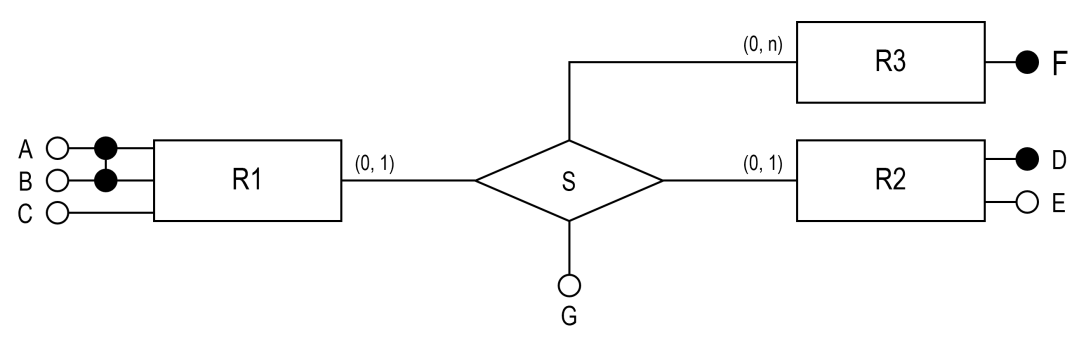
\includegraphics[width=0.8\linewidth]{tut_07_images/er_diag.png}
        % \caption{Caption}
        \label{fig:ERD}
    \end{figure}
\end{frame}

\begin{frame}{Q 2. Solution}
    \begin{figure}
        \centering
        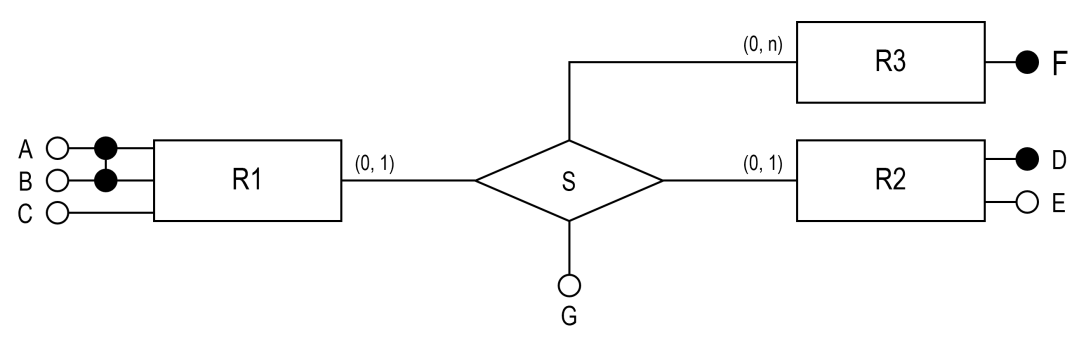
\includegraphics[width=0.6\linewidth]{tut_07_images/er_diag.png}
        % \caption{Caption}
        \label{fig:ERD2}
    \end{figure}
\small
\begin{itemize}
    \item From $R1$ we have $\{A,B\}\to C$.
    \item From $R2$ we have $\{D\}\to\{E\}$.
    \item From $R3$ we do not have anything extra.
    \item From participation of $R1$ and $R2$ in $S$, $\{A,B\} \to \{D\}$ and also $\{D\}\to \{A,B\}$. We also have $\{A,B\}\to\{G\}$ and $\{D\}\to \{G\}$.
    \item From participation of $R1$, $R2$ and $R3$ in $S$, we have $\{A,B\}\to \{F\}$, and $\{D\}\to \{F\}$.
\end{itemize}
\end{frame}

\begin{frame}{Codes}
\centering
    You can take a look at this repository that will help you create random FD problems for your practice, and also given a csv file, you can find functional dependencies:\\
    \href{https://github.com/pratik2358/fucntional_dep}{\textcolor{blue}{https://github.com/pratik2358/fucntional_dep}}
\end{frame}

\begin{frame}
\begin{center}
Questions?\\
Drop a mail at: pratik.karmakar@u.nus.edu
\end{center}
\end{frame}
\end{document}